Finden Sie eine Lösung der Differentialgleichung 
\begin{equation}
y''(x)\cdot\cos x=y(x)
\label{aufgabe3-dgl}
\end{equation}
in Form einer Reihe
\begin{equation}
y(x)
=
a_0 + a_1\cos x + a_2 \cos 2x + a_3 \cos3x+\dots
\label{aufgabe3-ansatz}
\end{equation}
von Kosinus-Funktionen.
Berechnen Sie die Koeffizienten bis $a_5$.

\begin{hinweis}
Die Lösung ist proportional zu $a_0$, Sie dürfen daher annehmen, dass
$a_0=1$.
Verwenden Sie ausserdem die Formeln
\[
\cos\alpha \cdot \cos\beta
=
\frac12\bigl(\cos(\alpha-\beta) + \cos(\alpha+\beta)\bigr)
\]
und Koeffizientenvergleich.
\end{hinweis}

\begin{loesung}
Wir berechnen die zweite Ableitung des Ansatzes
\begin{align*}
y''(x)
&=
-a_1\cos x - 2^2 a_2\cos 2x -3^2a_3\cos 3x-4^2a_4\cos4x-\dots
\\
y''(x)\cdot\cos x
&=
-a_1\cos x\cdot\cos x
-2^2a_2\cos2x\cdot\cos x
-3^2a_3\cos3x\cdot\cos x
-4^2a_4\cos4x\cdot\cos x
-\dots
\end{align*}
Die Produkte von Kosinus-Funktionen können mit der Formel
\[
\cos x \cdot \cos kx
=
\frac12\bigl(\cos (k-1)x + \cos(k+1)x\bigr)
\]
vereinfacht werden.
\begin{align*}
y''(x)\cdot\cos x
&=
-a_1\frac12(1+\cos2x)
-2^2a_2\frac12(\cos x + \cos3x)
-3^2a_3\frac12(\cos2x + \cos4x)
\\
&\qquad
-4^2a_4\frac12(\cos3x + \cos5x)
-\dots
\\
&=
-\frac{a_1}2
-2^2a_2\frac12
\cos x
-\frac12(a_1+3^2a_3)
\cos2x
-\frac12(a_2+4^2a_4)
\cos3x
\\
&\qquad
-\frac12(a_4+5^2a_5)
\cos4x
+\dots
\end{align*}
Durch Koeffizientenvergleich erhalten wir
\begin{align*}
a_0&=-\frac12 a_1         &&\Rightarrow& a_1 &=-2a_0
\\
a_1&=-2^2\frac12a_2       &&\Rightarrow& a_2 &=-\frac{2}{2^2}a_1
\\
a_2&=-\frac12(a_1+3^2a_3) &&\Rightarrow& a_3 &= -\frac{1}{3^2}(2a_2+a_1)
\\
a_3&=-\frac12(a_2+4^2a_4) &&\Rightarrow& a_4 &= -\frac{1}{4^2}(2a_3+a_2)
\\
a_4&=-\frac12(a_3+5^2a_5) &&\Rightarrow& a_5 &= -\frac{1}{5^2}(2a_4+a_3)
\end{align*}
Offenbar sind die Koeffizienten $a_k$ mit $k>0$ proportional zu $a_0$,
die Lösungsfunktion ist daher ein Vielfaches der Funktion, welche man
erhält, wenn man $a_0=1$ setzt.
Damit sind die ersten vier Koeffizienten sofort zu berechnen:
\begin{align*}
a_1&=-2\\
a_2&= 1\\
a_3&= 0
\end{align*}
Für die Koeffizienten $a_k$ mit grösseren $k$ verwenden wir die 
Rekursionsformel
\[
a_k=-\frac{1}{k^2}(2a_{k-1}+a_{k-2})
\]
und erhalten die Koeffizienten in Tabelle~\ref{aufgabe3-tabelle}.
\begin{table}
\centering
\begin{tabular}{>{$}l<{$}|>{$}r<{$}}
k&a_k\\
\hline
 0&   1\phantom{.000000000000000}\\
 1&  -2\phantom{.000000000000000}\\
 2&   1\phantom{.000000000000000}\\
 3&  \phantom{-}0\phantom{.000000000000000}\\
 4&  -0.0625\phantom{00000000000}\\
 5&   0.005\phantom{000000000000}\\
 6&   0.001458333333333\\
 7&  -0.000161564625850\\
 8&  -0.000017737563776\\
 9&   0.000002432589548\\
10&   0.000000128723847\\
11&  -0.000000022231713\\
12&  -0.000000000585142\\
13&   0.000000000138473\\
14&   0.000000000001572\\
15&  -0.000000000000629\\
16&  -0.000000000000001\\
17&   0.000000000000002\\
\end{tabular}
\caption{Tabelle der Koeffizienten für die
Lösungsfunktion~\eqref{aufgabe3-ansatz} der Differentialgleichung
\eqref{aufgabe3-dgl}.
\label{aufgabe3-tabelle}}
\end{table}
\begin{figure}
\centering
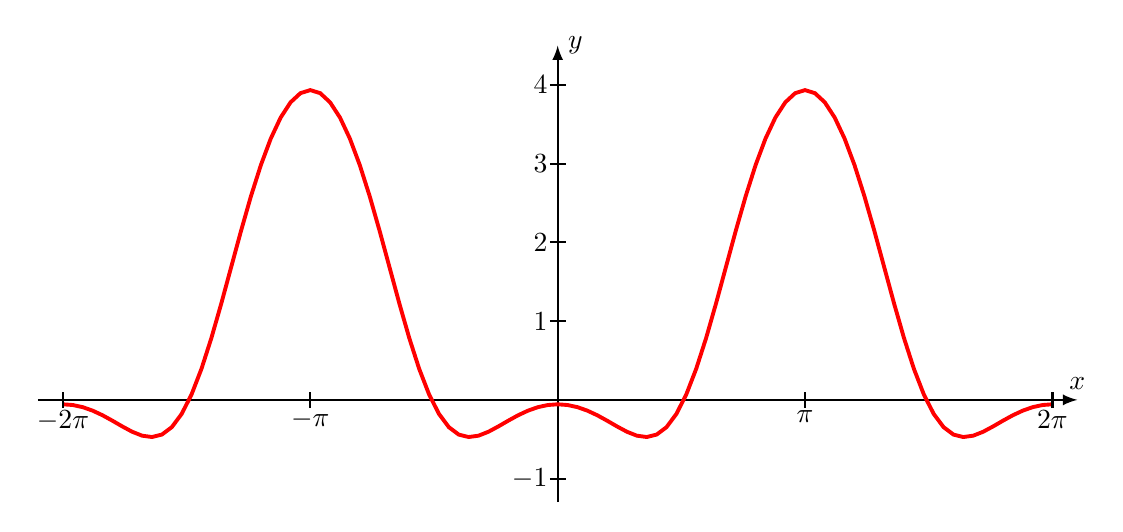
\begin{tikzpicture}[>=latex,thick]
\draw[->] (-6.6,0)--(6.6,0) coordinate[label=$x$];
\draw[->] (0,-1.3)--(0,4.5) coordinate[label={right:$y$}];
\draw (-0.1,1)--(0.1,1); \node at (0,1) [left] {$1$};
\draw (-0.1,2)--(0.1,2); \node at (0,2) [left] {$2$};
\draw (-0.1,3)--(0.1,3); \node at (0,3) [left] {$3$};
\draw (-0.1,4)--(0.1,4); \node at (0,4) [left] {$4$};
%\draw (-0.1,5)--(0.1,5); \node at (0,5) [left] {$5$};
\draw (-0.1,-1)--(0.1,-1); \node at (0,-1) [left] {$-1$};
\draw[domain=-360:360,samples=101,color=red,line width=1.4pt] plot
({3.1415*(\x)/180},{1-2*cos(\x) + cos(2*(\x)) -0.0625*cos(4*(\x))+0.005*cos(5*(\x)) +0.001458333*cos(6*(\x)) -0.000161564*cos(7*(\x)) -0.00001773*cos(8*(\x))});
\draw (-3.1415,-0.1)--(-3.1415,0.1);
\draw (3.1415,-0.1)--(3.1415,0.1);
\draw (-6.2830,-0.1)--(-6.2830,0.1);
\draw (6.2830,-0.1)--(6.2830,0.1);
\node at (-3.1415,0) [below] {$-\pi$};
\node at (3.1415,0) [below] {$\pi$};
\node at (6.2830,0) [below] {$2\pi$};
\node at (-6.2830,0) [below] {$-2\pi$};
\end{tikzpicture}
\caption{Graphische Darstellung der Lösungsfunktion der Differentialgleichung
\eqref{aufgabe3-dgl}.}
\end{figure}
\end{loesung}
